\documentclass[a4paper]{extarticle}
\usepackage[utf8]{inputenc}
\usepackage[a4paper, margin=1in]{geometry}

\usepackage{amssymb}
\usepackage{amsmath}
\usepackage{enumitem}
\usepackage{tcolorbox}
\usepackage{fancyhdr}
\usepackage{graphicx}
\usepackage{float}

\setlength{\parindent}{0em}
\setlength{\parskip}{0.4em}

\definecolor{theoremblue}{RGB}{1, 73, 124}
\definecolor{corollaryblue}{RGB}{70, 143, 175}
\definecolor{exampleblue}{RGB}{137, 194, 217}

\newtcolorbox{tbox}{colback=theoremblue!20,colframe=theoremblue,
boxrule=0pt,arc=0pt,boxsep=2pt,left=2pt,right=2pt,leftrule=2pt}

\newtcolorbox{cbox}{colback=corollaryblue!20,colframe=corollaryblue,
boxrule=0pt,arc=0pt,boxsep=2pt,left=2pt,right=2pt,leftrule=2pt}

\newtcolorbox{ebox}{colback=exampleblue!20,colframe=exampleblue,
boxrule=0pt,arc=0pt,boxsep=2pt,left=2pt,right=2pt,leftrule=2pt}

\title{IntroML - Lecture Notes Week 7}
\author{Ruben Schenk, ruben.schenk@inf.ethz.ch}
\date{\today}

\pagestyle{fancy}
\fancyhf{}
\rhead{ruben.schenk@inf.ethz.ch}
\rfoot{Page \thepage}
\lhead{IntroML - Lecture Notes Week 7}

\begin{document}

\maketitle

\subsection{Stochastic Gradient Descent for ANNs}

The \textbf{stochastic gradient descent} approach for ANNs looks as follows:

\begin{cbox}
    \textbf{Algorithm:} We want to solve
    \[
        W^* = \arg \min_{W} \sum_{i = 1}^n l(W; \, x_i, \, y_i)
    \]
    \begin{enumerate}
        \item We initialize the weight $W$
        \item For $t = 1, \, 2,...$:
        \begin{itemize}
            \item Pick data point $(x, \, y) \in D$ uniformly at random
            \item Take step in \textit{negative gradient} direction
            \[
                W \leftarrow W - \eta \Delta_Wl(W; \, x, \, y)
            \]
        \end{itemize}
    \end{enumerate}
    Typically we use \textit{minibatches} to reduce variance/exploit parallelization.
\end{cbox}

But how do we optimize over weights? We want to do \textbf{empirical risk minimization,} i.e. jointly optimize over all weights for all layers to minimize loss over the training data. This is in general a \textit{non-convex} optimization problem! Nevertheless, we can still try to find a local optimum.

\textbf{Remark:} There are \textbf{weight-space symmetries.} Multiple distinct weights can compute the same predictions. In other words, multiple local minima can be equivalent in terms of input-output mapping.

Computing the gradient is done through backpropagation in matrix form:

\begin{cbox}
    \textbf{Algorithm:}
    \begin{enumerate}
        \item For the output layer
        \begin{itemize}
            \item Compute "error": $\delta^{(L)} = \Delta_fl$
            \item Gradient: $\Delta_{W^{(L)}}l = \delta^{(L)}v^{(L-1)T}$
        \end{itemize}
        \item For each hidden layer $l = L - 1:-1:1$
        \begin{itemize}
            \item Compute "error": $\delta^{(l)} = \phi'(z^{(l)})\odot (W^{(l + 1)T}\delta^{(l+1)})$
            \item Gradient: $\Delta_{W^{(l)}}l = \delta^{(l)}v^{(l-1)T}$
        \end{itemize}
    \end{enumerate}
\end{cbox}

\subsection{Weight Initialization in Neural Networks}

Onr problem we might encounter are \textbf{vanishing} and \textbf{exploding gradients.} Remember the gradient computation in backpropagation was defined as:
\[
    \Delta_{W^{(i)}}l = \delta^{(i)}v^{(i - 1)T} \text{ where } \delta^{(i)} = \phi'(z^{(i)}) \odot (W^{(i + 1)T}\delta^{(i + 1)}) \text{ and } v^{(i)} = \phi(W^{(i)}v^{(i-1)})
\]
The potential issue is exploding ($||\Delta_{W^{(i)}}l|| \to \infty$) or vanishing ($||\Delta_{W^{(i)}}l|| \to 0$) gradients can cause optimization to fail. Why can this happen? Potential reasons are $||\delta^{(i)}||$ going to $0$ or $\infty$ (or analog. for $||v^{(i)}||$).
\begin{itemize}
    \item Using certain activation functions (e.g. ReLU) can help avoid $||\delta^{(i)}|| \to 0$.
    \item The error signal $\delta^{(i)}$ is scaled by $v^{(i)}$. This can help to reduce the vanishing/exploding gradient problem by keeping the magnitude of $v^{(i)}$ constant across the layers.
\end{itemize}

The general goal when initializing weights is to keep the variance of weights approximately constant across layers to avoid vanishing and exploding gradients and network activations. Usually, \textbf{random initialization} works well, e.g.
\begin{itemize}
    \item Glorot ($\tanh$): $w_{i, \, j} \sim \mathcal{N}(\frac{1}{n_{in}})$ or $w_{i, \, j} \sim \mathcal{N}(\frac{2}{n_{in} + n_{out}})$
    \item He (ReLU): $w_{i, \, j} \sim \mathcal{N}(\frac{2}{n_{in}})$
\end{itemize}
We need to ensure that at initialization, unit activations are approximately standardized.

\subsection{Learning Rates}

To implement the SGD update rule ($W \leftarrow W - \eta_t\Delta_Wl(W; \, x, \, y)$), we need to choose the learning rate $\eta_t$. In practice, we often use a decaying learning rate schedule, e.g. piecewise constant.

We may want to monitor the ratio of weight change (gradient) to weight magnitude:
\begin{itemize}
    \item If it's too small, we increase the learning rate
    \item If it's too large, we decrease the learning rate
\end{itemize}

\textbf{Learning with momentum} is a common extension to training with (stochastic) gradient descent. It can help to escape the local minima. The idea is as follows: We move not only into the direction of the gradient, but also in direction of the last weigh update. The updates then are:
\begin{itemize}
    \item $d \leftarrow m \cdot d + \eta_t\Delta_Wl(W; \, x, \, y)$
    \item $W \leftarrow W - d$
\end{itemize}
In some cases, learning with momentum cad \textit{prevent oscillation.}

\subsection{Recularization in Neural Networks}

Neural networks have many parameters, so there's a potential danger of overfitting. Countermeasures are:
\begin{itemize}
    \item \textit{Regularization (weight decay):} Add penatly term to keep the weights small
    \[
        W^* = \arg \min_W \sum_{i = 1}^n l(W; \, x_i, \, y_i) + \lambda ||W||_2^2
    \]
    \item \textit{Early stopping:} Don't run SDG until convergence
    \item \textit{"Dropout"}
\end{itemize}

The idea behind \textbf{early stopping} is as follows: In general, we might not want to run the training until the weights convergence since this potentially leads to overfitting. One posssibility is:
\begin{enumerate}
    \item Monitor the prediction perfomance on a validation set
    \item Stop the training once the valdiation error stops to decrease
\end{enumerate}

The idea behind the \textbf{dropout} technique is to randomly ignore hidden units during each iteration of SGD with probability $p$:

\begin{figure}[H]
    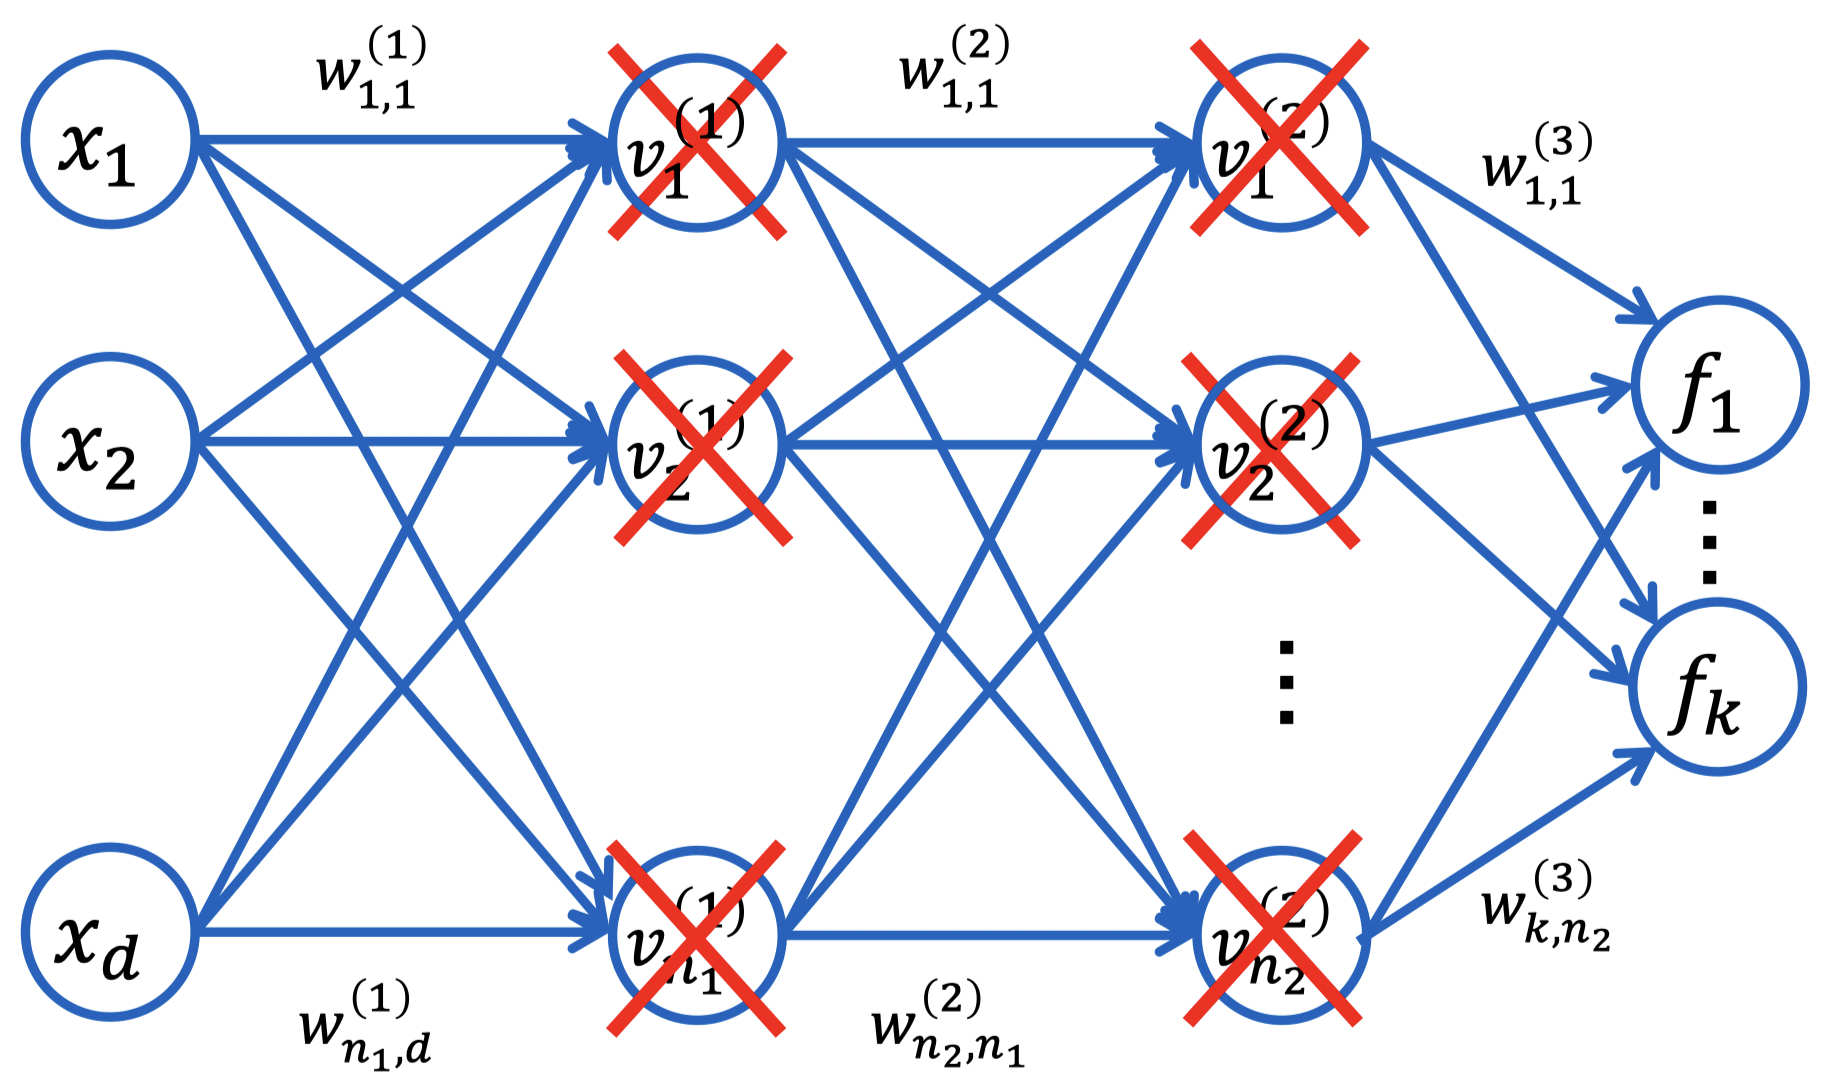
\includegraphics[width=15cm]{../images/IntroML_Fig7-1}
    \centering
\end{figure}

After the training, we use all units, but multiply the weights by $p$ to compensate.

\begin{figure}[H]
    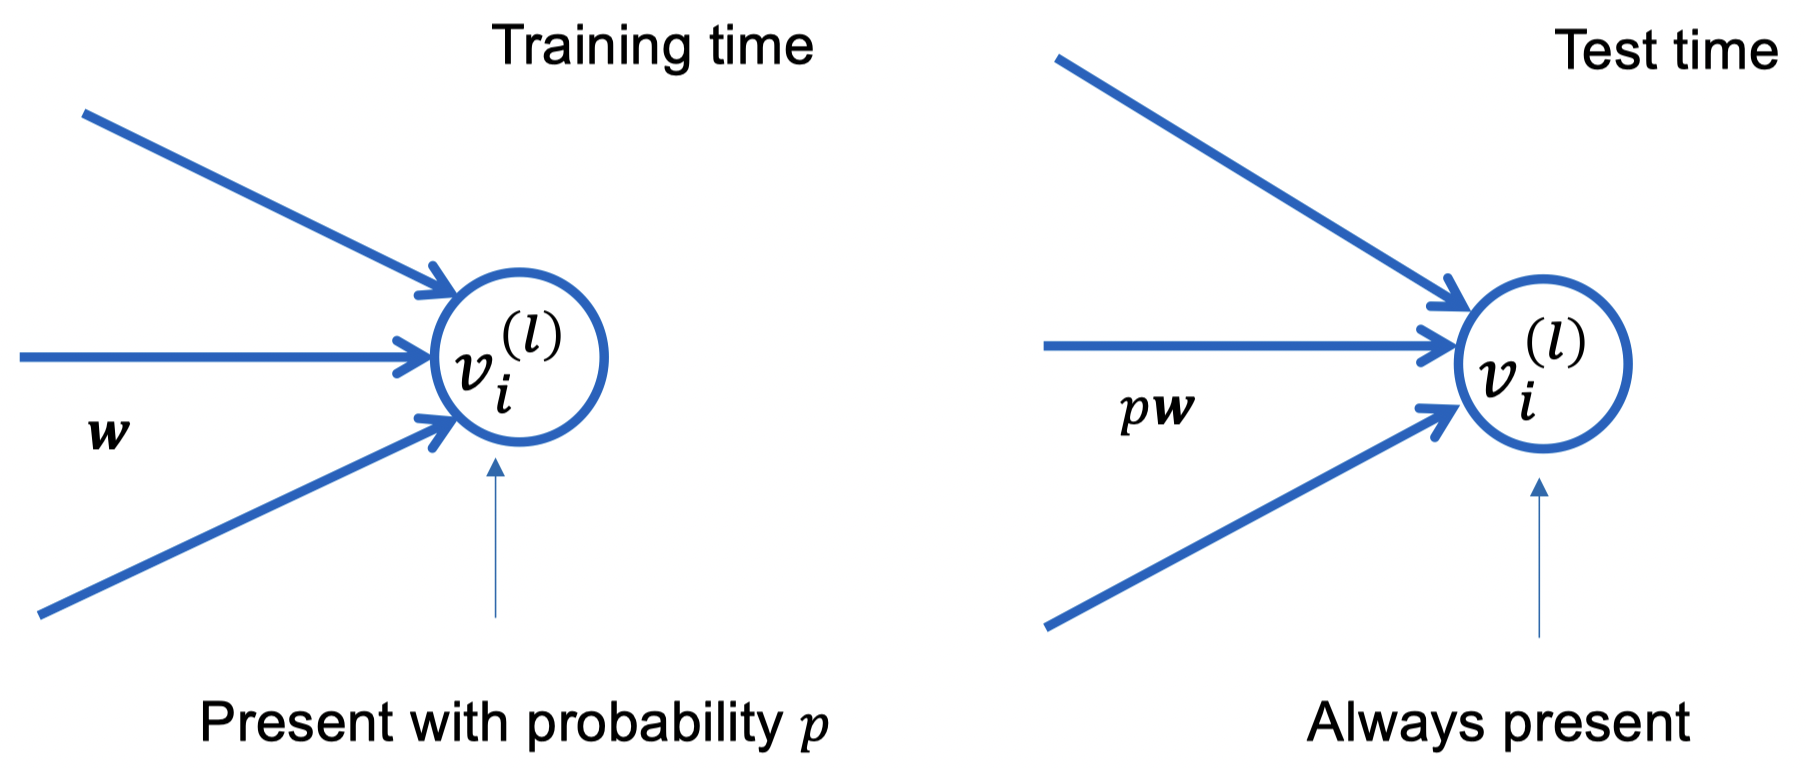
\includegraphics[width=15cm]{../images/IntroML_Fig7-2}
    \centering
\end{figure}

\subsection{Batch Normalization}

In deep learning, inputs are shifted and scaled through each layer. \textbf{Batch normalization} is a widely used technique that normalizes unit activations in each layer according to mini-batch statistics:
\begin{itemize}
    \item Reduces internal covariate shift
    \item Enables larger learning rates
    \item Has regulatizing effect
\end{itemize}
This can be integrates as a layer into the neural network, with two learnable parameters $\beta, \, \gamma$ (per hidden unit) that can "learn to undo" the normalization (and also serve as bias nodes).

This encourages standardization of unit activations not only for inputs, but also hidden units. Not only at initialization, but also during training.

\begin{cbox}
    \textbf{Algorithm:} Batch normalization layer
    \begin{enumerate}
        \item Input: Incoming activation values for all examples $v_i$ for all $i \in S$ in the minibatch $S$, $\epsilon > 0$
        \item Learnable parameters: $\beta, \, \gamma$
        \item Batch normalization computes $\bar{v} = BN(v; \, \gamma, \, \beta)$ by:
        \begin{enumerate}
            \item Compute the mini-batch mean: $\mu_S = \frac{1}{|S|} \sum_{i \in S}v_i$
            \item Compute the mini-batch variance: $\sigma_S^2 = \frac{1}{|S|} \sum_{i \in S} (v_i - \mu_S)^2$
            \item Normalize each point: $\hat{v}_i = \frac{v_i - \mu_s}{\sqrt{\sigma_S^2 + \epsilon}}$
            \item Scale and shift: $\bar{v}_i = \gamma \hat{v}_i + \beta$
        \end{enumerate}
        \item Output: $\bar{v}_i$ for all $i \in S$ in the minibatch $S$
    \end{enumerate}
\end{cbox}

\section{Convolutional Neural Networks}

\subsection{Introduction}

So far, we have only discussed fully connected neural networks. There exist, however, specialized archtiectures designed for certain classes of applciations, such as:
\begin{itemize}
    \item Convolutional neural networks
    \item Residual networks and skip connections
    \item Recurrent neural networks
    \item Memory (LSTMs, GRUs,...)
    \item etc.
\end{itemize}

Let us pose some invariances of predictions. Predictions should be unchanged under some transformations of the data, e.g.:¨
\begin{itemize}
    \item Classifications of handwritten digits should be undchanged under translation, rotation, scale, etc.
    \item Speech recognition
\end{itemize}

How do we encourage a model to learn specific invariances?
\begin{itemize}
    \item Augmentation of the training set
    \item Special regularization terms
    \item Invariance built into pre-processing
    \item Implement invariance into structure of ANN (e.g. using convolutional neural networks)
\end{itemize}

\subsection{Convolutions}

\textbf{Convolutional neural networks} are ANNs for \textit{specialized applications} (e.g. image recognition). The hidden layers closest to the input layer \textit{share parameters:} Each hidden unit only depends on all closeby inputs (e.g. pixels), and weights constrained to be identical across all units on the layer. This reduces the number of parameters, and ecnourages robustness against small amounts of translation.

\textbf{Remark:} The weights can still be optimized via backpropagation.

Lets first consider convolutions in 1D. We can define this as follows: Given a row vector $w \in \mathbb{R}^k$ and a column $x \in \mathbb{R}^d$, then their \textbf{convolution} $z = w * x$ is defined by the vector $z \in \mathbb{R}^{d + k - 1}$ via
\[
    z_i = \sum_{j = \max(1, \, i - d + 1)}^{\min (i, \, k)} w_jx_{i-j+1}.
\]
This naturally generalizes to matrices $W$ to yield $z = W * x$.

Lets also consider convolutions with 2D data (such as images). We summarize the approach in the following figure:

\begin{figure}[H]
    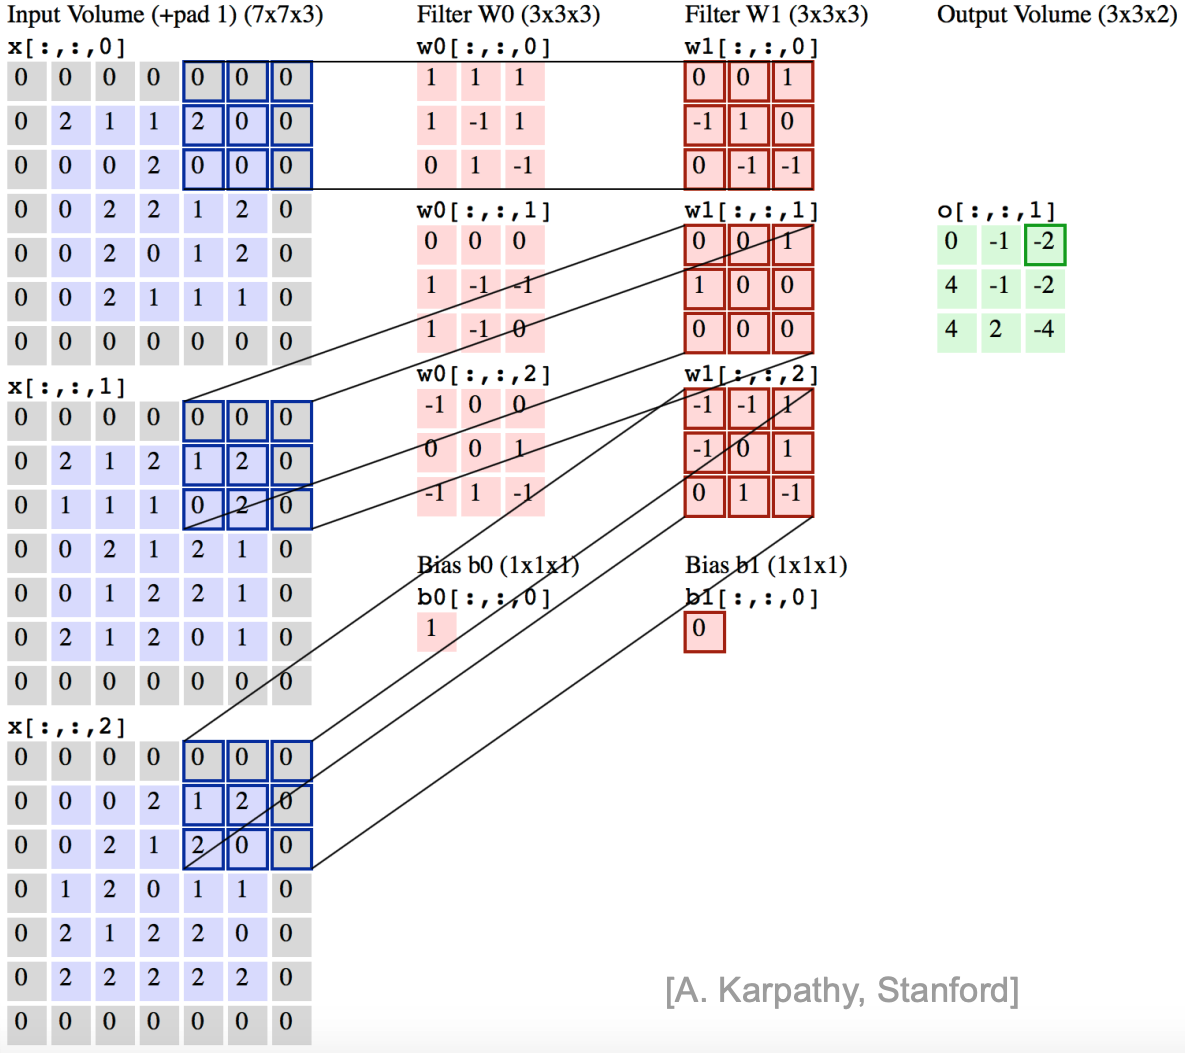
\includegraphics[width=15cm]{../images/IntroML_Fig7-3}
    \centering
\end{figure}

If we compare those to fully connected layers, we see the following similarities:
\begin{itemize}
    \item Fully connected layers: $v^{l + 1} = \phi(Wv^l)$
    \item Convolutional layers: $v^{l + 1} = \phi(W * v^l)$
\end{itemize}

We might also be interested in computing the \textit{output dimensions:}
\begin{itemize}
    \item Apply $m$ different $f \times f$ filters
    \item To a $n \times n$ image
    \item With PAdding $p$
    \item And stride $s$
\end{itemize}
Then:
\[
    l = \frac{n + 2p - f}{s} + 1
\]

\subsection{CNN Architecture}

Finally, this leaves us with the following architecture for CNNs:

\begin{figure}[H]
    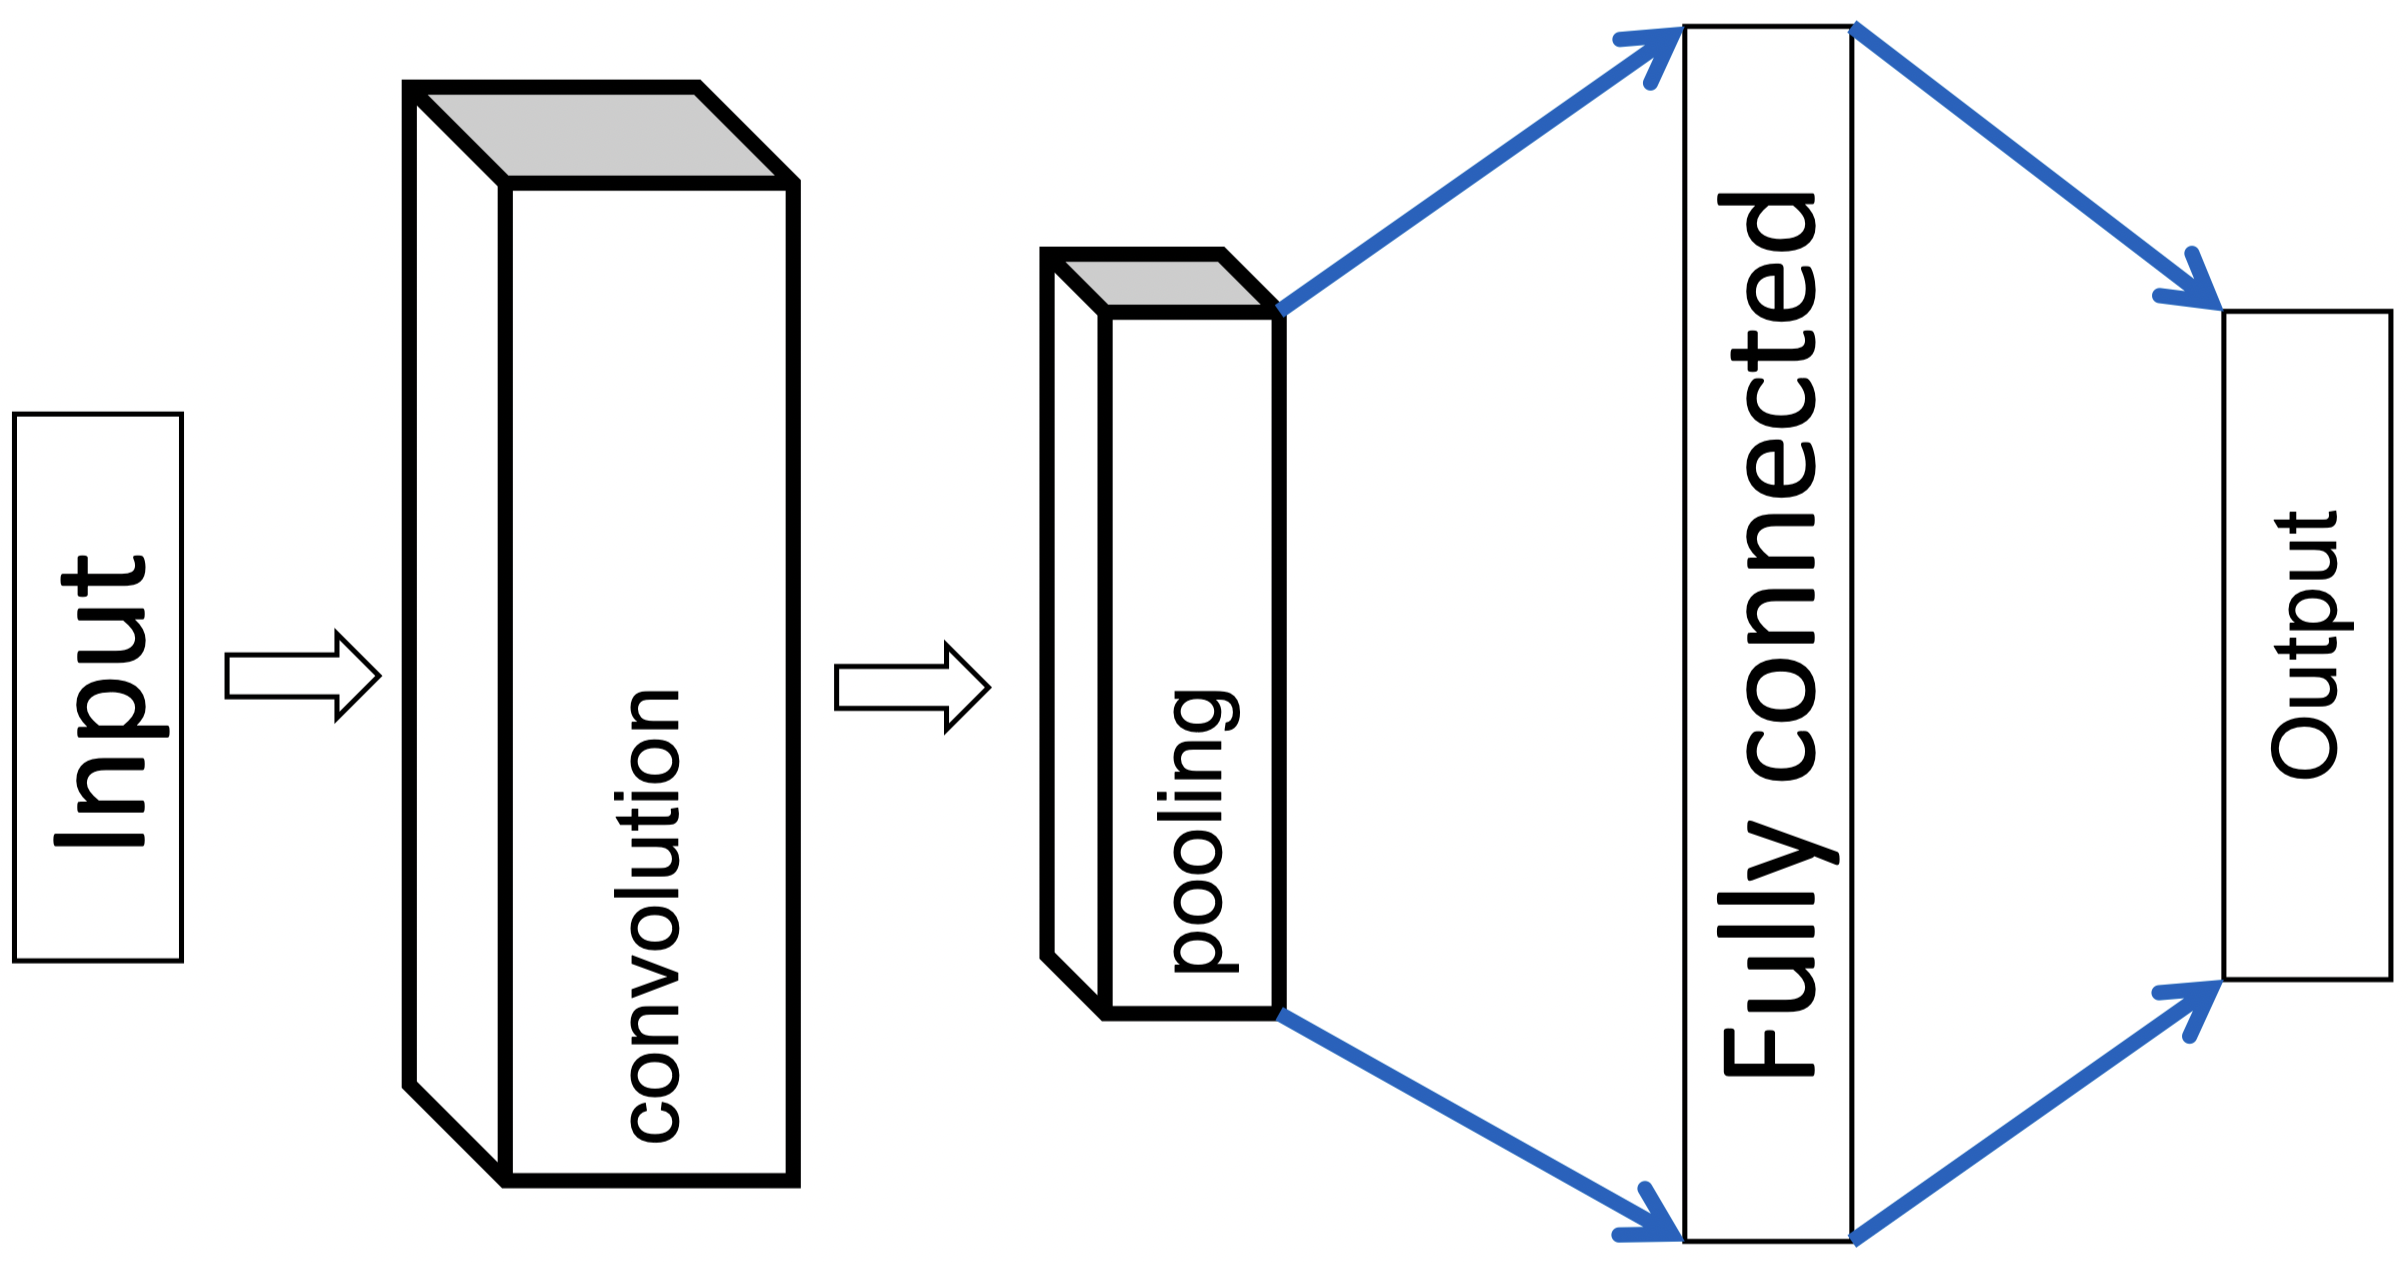
\includegraphics[width=15cm]{../images/IntroML_Fig7-4}
    \centering
\end{figure}

In some applications, it can make sense to \textbf{aggregate (pool)} several units to decrease the width of the network (and hence the number of parameters). Usually, one considers either the average or the maximum value. Example:

\begin{figure}[H]
    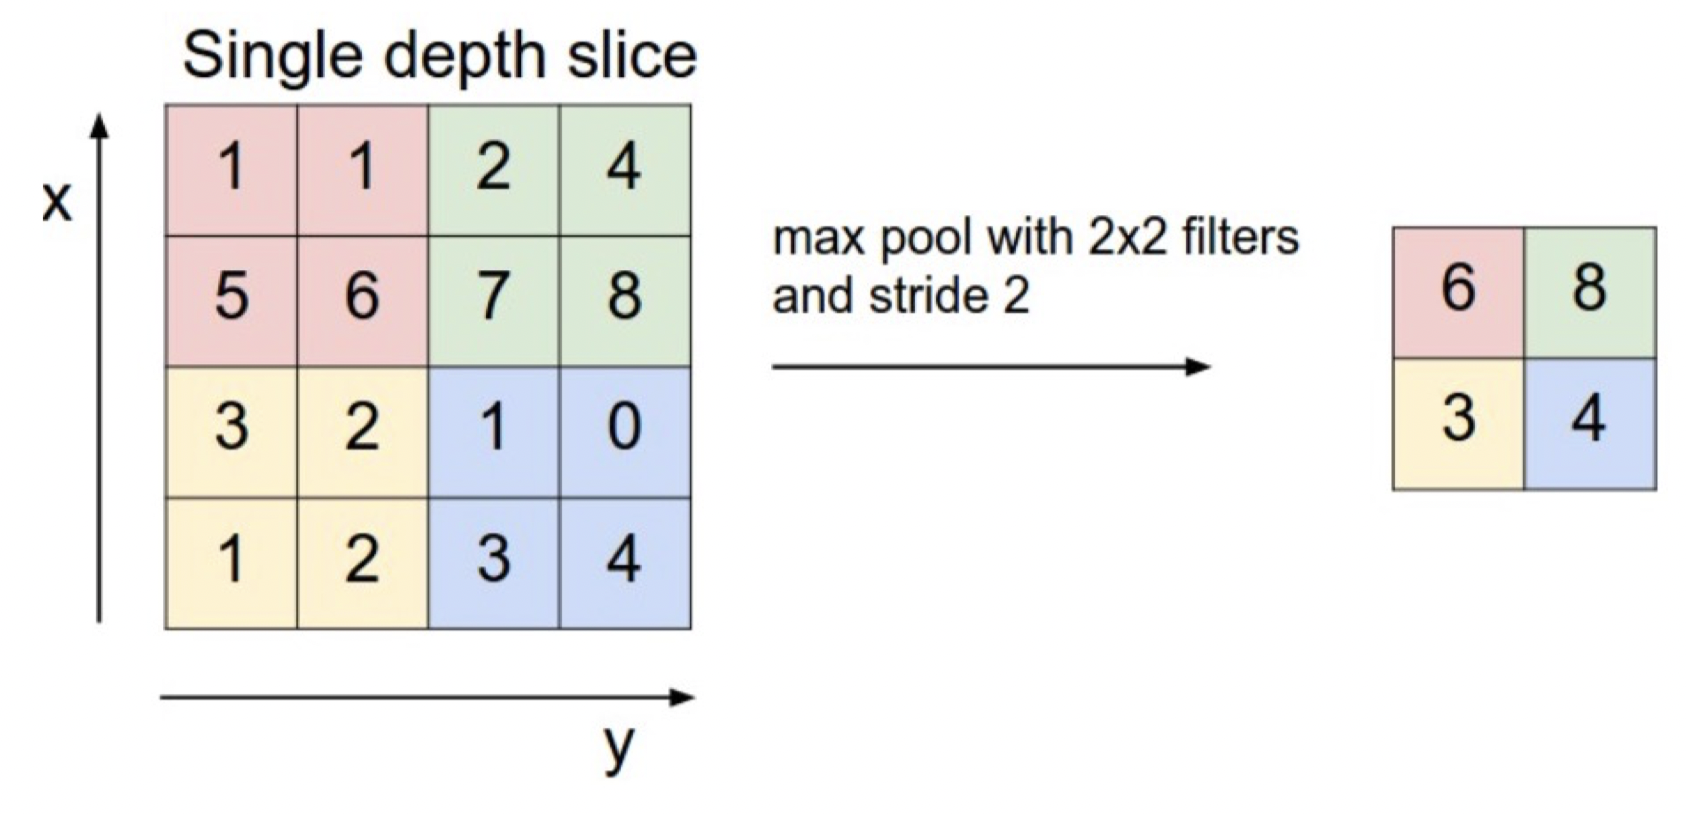
\includegraphics[width=13cm]{../images/IntroML_Fig7-5}
    \centering
\end{figure}

\begin{figure}[H]
    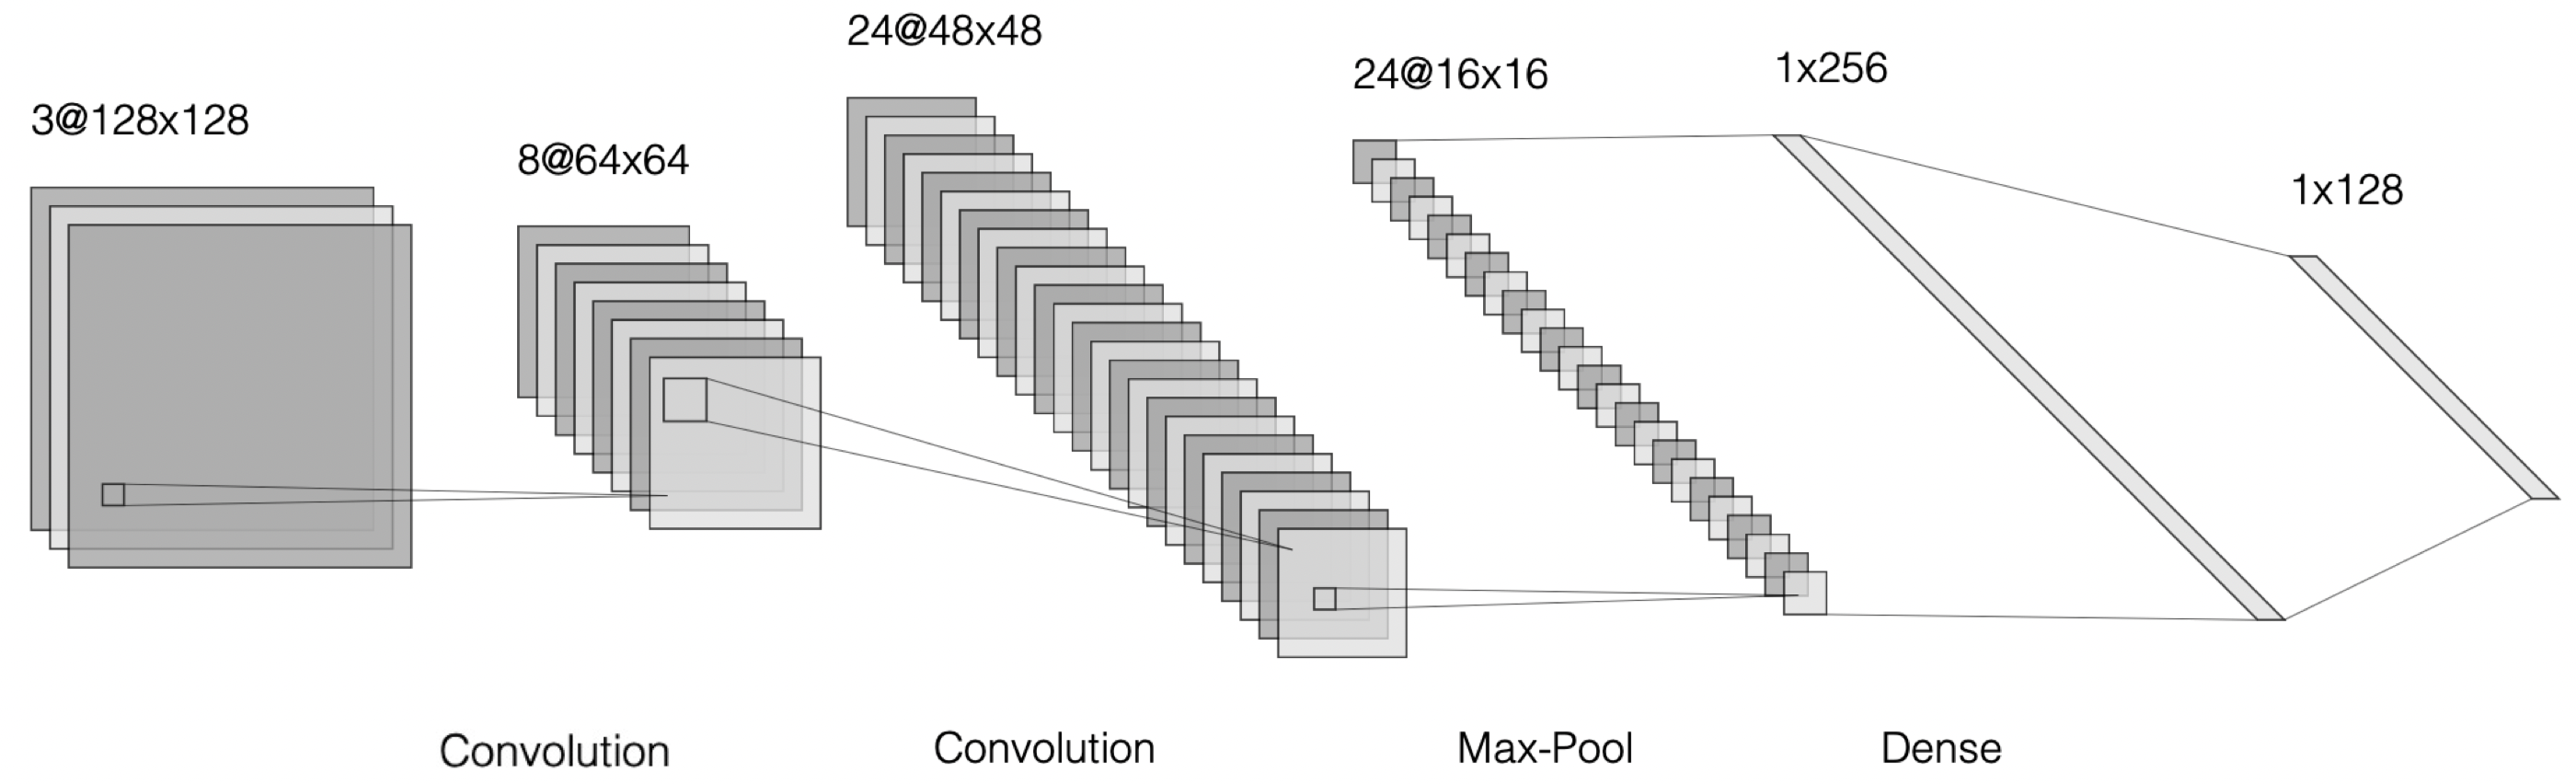
\includegraphics[width=15cm]{../images/IntroML_Fig7-6}
    \centering
\end{figure}

\subsection{Residual Networks}

\begin{figure}[H]
    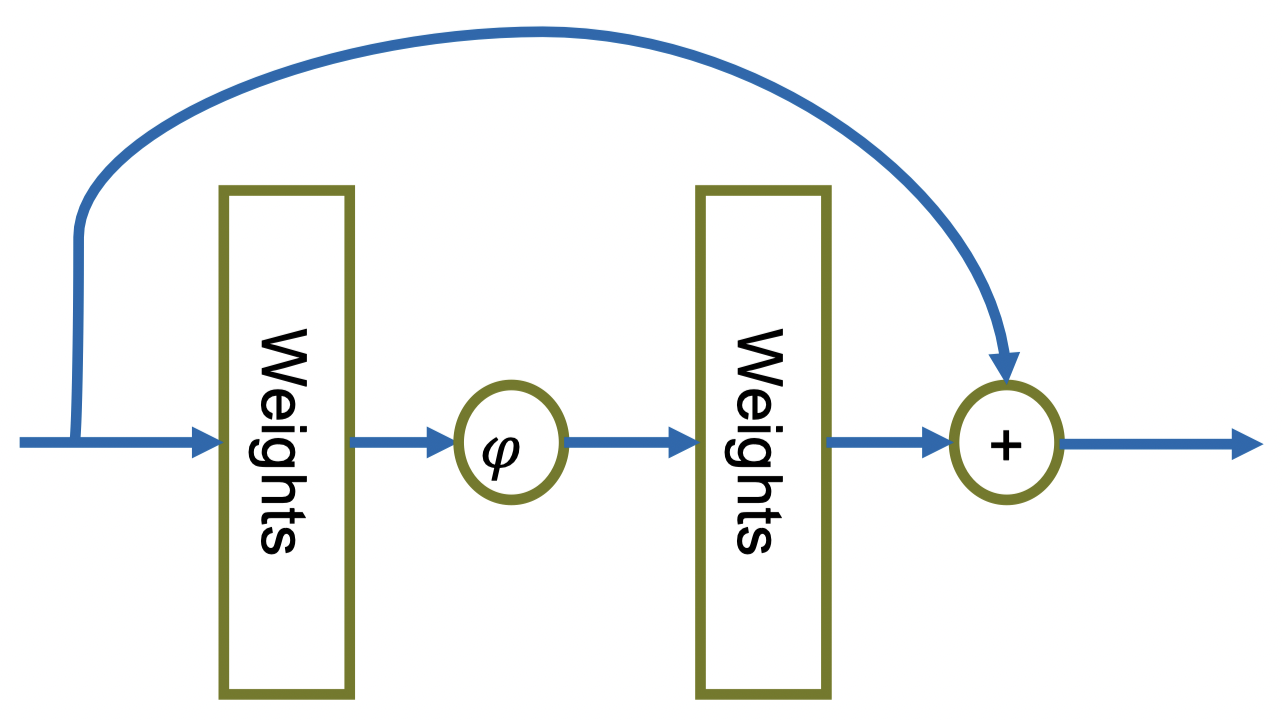
\includegraphics[width=9cm]{../images/IntroML_Fig7-7}
    \centering
\end{figure}

The idea behind \textbf{residual connections} is as follows:
\begin{enumerate}
    \item Introduce skip connections that can allow to effectively train deeper networks
    \item "Identity shortcut connection" helps to avoid vanishing gradients
    \item This allows to effectively train networks with 1000+ layers
    \item It's also possible to skip more than one layer (DenseNets)
\end{enumerate}

\end{document}